\section{Ordinary cluster algebras}\label{sec:ordinaryClusterAlgebras}

Cluster algebras were originally introduced in 2000 by Fomin and Zelevinsky~\cite{Fomin-Zelevinsky-I} to provide a concrete combinatorial framework for studying dual canonical bases and total positivity in semisimple groups. Cluster algebras are commutative rings with a distinguished family of ge\-nerators, called \emph{cluster variables}, which occur in distinguished collections of $n$-element subsets $\{x_1, \dots, x_n \}$ called \emph{clusters}. Clusters can be obtained from each other by an involutive process called \emph{mutation}, which replaces a single cluster variable with a unique cluster variable which was not present in the original cluster. Through repeated mutation, one can recover the complete set of cluster variables.

Algebraically, mutation is given by a binomial \emph{exchange relations}. The coefficients in these binomial exchange relations come from a choice of \emph{coefficient variables}. Each cluster $\{ x_1, \dots, x_n \}$ has an associated set of coefficients $\{y_1, \dots, y_n \}$, which are also related to each other via mutation. For more technical definitions, one good source is \cite[Section~2]{Fomin-Zelevinsky-IV}.

Cluster algebras have a variety of notable properties -- these famously include the \emph{Laurent phenomenon}.

\begin{Theorem}[{\cite[Theorem 3.1]{Fomin-Zelevinsky-I}}]
Let $\mathcal{A}$ be an arbitrary cluster algebra. The cluster variables $x_1, \dots, x_n$ can be expressed in terms of any cluster of~$\mathcal{A}$ as a Laurent polynomial with coefficients in~$\mathbb{ZP}$.
\end{Theorem}

The Laurent phenomenon becomes even more compelling with the addition of the \emph{positivity property}.

\begin{Conjecture}[{cf.\ \cite[Section 3]{Fomin-Zelevinsky-I}}]
The coefficients of these Laurent polynomials are in fact \emph{non-negative}.
\end{Conjecture}

Positivity was conjectured in Fomin and Zelevinsky's original paper \cite{Fomin-Zelevinsky-I} and later verified in a variety of cases, including: skew-symmetric cluster algebras \cite{Lee-Schiffler}, cluster algebras of surface type \cite{MSW, Schiffler, Schiffler-Thomas}, acyclic (quantum) cluster algebras \cite{Caldero-Reineke, Efimov,Kimura-Qin, Qin}, bipartite cluster algebras \cite{Nakajima}, and cluster algebras of geometric type~\cite{GHKK}. Note that this last case encompasses all of the prior cases and is the most general setting in which a proof of the positivity conjecture is known.

Throughout, we will use the term \emph{ordinary cluster algebra} to refer to this original definition due to Fomin and Zelevinsky.

\subsection{Cluster algebras from surfaces}

In 2008, Fomin, Shapiro, and D.~Thurston showed that a subset of ordinary cluster algebras can be modeled by triangulations of bordered surfaces with marked points~\cite{FST-triangulatedSurfaces}. Marked points that appear on the interior of the surface are called \emph{punctures}. We work primarily with unpunctured surfaces, but will note some connections to punctures in Section~\ref{sec:RelateToPuncture}. For unpunctured surfaces, we quickly highlight some relevant portions of Fomin, Shapiro, and D.~Thurston's construction and refer the reader to Section~2 of their paper for a much more detailed explanation.

\begin{Definition}An \emph{arc} $\gamma$ on a surface $(S,M)$ is a non-self-intersecting curve in $S$ with endpoints in $M$ that is otherwise disjoint from $M$ and $\partial S$. Curves that are contractible onto $\partial S$ or that cut out an unpunctured monogon or bigon are not considered arcs. Arcs are considered up to isotopy class.
\end{Definition}

Because arcs are considered up to isotopy, we have to be somewhat careful when thinking about the idea of intersections of arcs. Let $\gamma$ and $\gamma'$ be arbitrary arcs on $S$ and $\alpha$ and $\alpha'$ denote arbitrary representatives of their isotopy classes. Then the \emph{crossing number} $e(\gamma,\gamma')$ is the minimal number of crossings of each possible choice of $\alpha$ and $\alpha'$. Two arcs $\gamma$ and $\gamma'$ are considered \emph{compatible} if $e(\gamma,\gamma') = 0.$ Similarly, if $T = \{\tau_1,\ldots,\tau_n\}$ is a triangulation of a surface, we define $e(\gamma,T) = \sum_{i=1}^n e(\gamma, \tau_i)$.

\begin{Definition}
An \emph{ideal triangulation} $T$ of a surface is a maximal collection of pairwise compatible arcs (and boundary arcs).
\end{Definition}

Surfaces with ideal triangulations provide a useful combinatorial tool for studying certain cluster algebras, via the correspondence described in the following theorem.

\begin{Theorem}[Fomin--Thurston \cite{FT-II}]\label{SurfaceCA}
Given a surface with marked points, $(S,M)$, there exists a unique cluster algebra $\mathcal{A} = \mathcal{A}(S,M)$ with the following properties: $(1)$~the seeds are in bijection with tagged triangulations of $(S,M)$;
$(2)$~the cluster variables are in bijection with tagged arcs in $(S,M)$; and $(3)$~the cluster variable $x_\gamma$ corresponding to arc $\gamma$ is given by the lambda length of $\gamma$, in terms of some initial triangulation.
\end{Theorem}
 In this dictionary, mutation of cluster variables in $\mathcal{A}$ is equivalent to flipping arcs in the triangulation~$T$. Each arc $\tau$ in $T$ looks locally like the diagonal in a quadrilateral. Thus, the result of flipping $\tau$ in $T$ is a new triangulation, $T' = (T - \{\tau\}) \cup \{\tau' \}$ where $\tau'$ is the unique other diagonal of the quadrilateral surrounding $\gamma$.

\subsection{Snake graphs}\label{section:snakeGraphs}

Snake graphs were defined by Musiker, Schiffler, and Williams in order to give explicit combinatorial formulas for the cluster variables in any cluster algebra from a surface \cite{MSW}. In doing so, they offered an alternate and combinatorial proof of positivity for cluster algebras from surfaces. For any fixed arc $\gamma$ and triangulation $T$ of a surface $(S,M)$, they construct a graph $G_{T,\gamma}$ by gluing together \emph{tiles} that encode the local geometry at each intersection between $\gamma$ and arcs of the triangulation. The formula for the expansion of $x_\gamma$ with respect to the cluster corresponding to $T$ is then given in terms of perfect matchings of $G_{T,\gamma}$. We briefly review their construction for unpunctured surfaces, but refer the interested reader to Section 4 of their paper for the complete construction and many examples.

Let $(S,M)$ be a bordered surface with triangulation $T$ and $\gamma$ be an ordinary arc (i.e., one without self-intersections) in $S$ but not in $T$. Fix an orientation on $\gamma$ and let $s$ and $t$ denote the starting and ending points of $\gamma$, respectively. Denote the intersection points of $\gamma$ and $T$ as $s = p_0, p_1, \dots, p_{d+1} = t$, in order, and let $\tau_{i_j}$ be the arc in $T$ containing $p_j$. Denote the ideal triangles on either side of $\tau_{i_j}$ as $\Delta_{j-1}$ and $\Delta_j$.

Each intersection $p_j$ is associated with a square tile $G_j$ formed by gluing copies of~$\Delta_{j-1}$ and~$\Delta_j$ along the edge labeled $\tau_{i_j}$. This can be done either so that both triangles have orientation matching~$\Delta_{j-1}$ and~$\Delta_j$ or both triangles have opposite orientation, hence there are two valid planar embeddings of each~$G_j$. The tile $G_j$ is said to have \emph{relative orientation} $\operatorname{rel}(G_j) = +1$ if the orientation of its triangles match the ideal triangles on $S$ and $\operatorname{rel}(G_j) = -1$ otherwise. Two of the edges of the triangle $\Delta_j$ are labeled $\tau_{i_j}$ and $\tau_{i_{j+1}}$; label the remaining edge as $\tau_{[\gamma_j]}$.

{\sloppy The graph $G_{T,\gamma}$ is then formed by gluing together subsequent tiles $G_{1}, \dots, G_{d}$ in order. Ti\-les~$G_j$ and~$G_{j+1}$ are glued along the edge labeled $\tau_{[\gamma_j]}$ after choosing planar embeddings~$\widetilde{G}_j$ and~$\widetilde{G}_{j+1}$ of the tiles such that $\operatorname{rel}\big(\widetilde{G}_j\big) \neq \operatorname{rel}\big(\widetilde{G}_{j+1}\big)$. Gluing together all~$d$ tiles gives a~graph~$\bar{G}_{T,\gamma}$. The graph $G_{T,\gamma}$ can then be obtained from $\bar{G}_{T,\gamma}$ by removing the diagonal edge from each tile.

}

Before stating Musiker, Schiffler, and Williams' expansion formula, we need to review the following definitions and notation.

\begin{Definition}[{\cite[Definition 4.4]{MSW}}]
For an ordinary arc $\gamma$ crossing the sequence of arcs $\tau_{i_1},\dots,\tau_{i_d}$ in $T$, the \emph{crossing monomial} of $\gamma$ with respect to $T$ is defined as
\begin{gather*}
\operatorname{cross}(T,\gamma) = \prod_{j=1}^d x_{\tau_{i_j}}.
\end{gather*}
\end{Definition}

\begin{Definition}[{\cite[Definition 4.5]{MSW}}]
A perfect matching $P$ of a snake graph $G$ which uses edges labeled $\tau_{i_1}, \dots, \tau_{i_k}$ has \emph{weight} $x(P) = x_{\tau_{i_1}}\cdots x_{\tau_{i_k}}$.
\end{Definition}

\begin{Definition}[{\cite[Definition 4.6]{MSW}}]\looseness=-1
$G_{T,\gamma}$ has exactly two perfect matchings that include only boundary edges; these are referred to as the \emph{minimal} and \emph{maximal} matchings of $G_{T,\gamma}$. The distinction between the two depends on the relative orientation of $G_{T,\gamma}$; if $\operatorname{rel}(G_{T,\gamma}) = 1$ (respectively, $-1$), define $e_1$ and~$e_2$ to be the edges that are immediately counterclockwise (respectively, clockwise) from the diagonal. The \emph{minimal matching}, $P_{-}$, is defined to be the unique perfect matching that includes only boundary edges and does not include $e_1$ or $e_2$. The \emph{maximal mat\-ching} $P_{+}$ is the complementary perfect matching on boundary edges that includes~$e_1$ and~$e_2$.
\end{Definition}

The cluster expansion formula from snake graphs involves the symmetric difference of an arbitrary perfect matching $P$ with $P_{-}$, denoted $P \ominus P_{-}$. The edges of $P \ominus P_{-}$ are always a~subgraph of $G_{T,\gamma}$ composed of potentially disjoint cycles, which encloses a finite set of tiles~$\{ G_{i_j} \}_{j \in J}$.

\begin{Definition}[{\cite[Definition 4.8]{MSW}}]
Let $T = \{ \tau_1, \dots, \tau_n \}$ be an ideal triangulation of an unpunctured surface $(S,M)$ and $\gamma$ be an ordinary arc on $(S,M)$. Let $P$ be a perfect matching of $G_{T,\gamma}$ such that $P \ominus P_{-}$ encloses the set of tiles $\{ G_{i_j} \}_{j \in J}$. The \emph{height monomial} of $P$ is
\begin{align*}
y(P) = \prod_{k=1}^n h_{\tau_{k}}^{m_k},
\end{align*}
where $m_k$ is the number of tiles in $\{G_{i_j} \}_{j \in J}$ with diagonal labeled $\tau_{i_j}$ and $h_{\tau_k} = y_{\tau_k}$.
\end{Definition}

Now, we are prepared to state the formula for obtaining Laurent expansions from snake graphs.

\begin{Theorem}[{\cite[Theorem 4.9]{MSW}}]\label{theorem:clusterExpansion_ordinary}
Let $(S,M)$ be a bordered surface with triangulation~$T$, $\mathcal{A}$~be the corresponding cluster algebra with principal coefficients, and~$\gamma$ be an ordinary arc on~$S$. Then $x_\gamma$ can be written as a Laurent expansion in terms of the initial cluster variables as
\[ x_\gamma = \frac{1}{\operatorname{cross}(T,\gamma)}\sum_P x(P)y(P), \]
where the sum ranges across all perfect matchings $P$ of the snake graph $G_{T,\gamma}$.
\end{Theorem}

Subsequently, Musiker and Williams extended the snake graph construction to handle \emph{generalized arcs}, which may contain self-intersections, and closed curves \cite{MW}. Suppose $\gamma$ is now a generalized arc. If $\gamma$ is a contractible loop, then Musiker and Williams define $x_\gamma = 0$. If $\gamma$ contains a contractible kink and $\overline{\gamma}$ denotes the corresponding arc with the kink removed, then they define $x_\gamma = (-1)x_{\overline{\gamma}}$. Musiker and Williams then show that Theorem \ref{theorem:clusterExpansion_ordinary} holds for generalized arcs. For closed curves, they define a corresponding cluster algebra element using a slight modification of snake graphs called \emph{band graphs}. For details, see \cite[Section~3]{MW}.

The set of perfect matchings of a snake graph has a natural poset structure. Describing this structure makes use of \emph{twists}, i.e. local moves on a perfect matching $P$ where the horizontal edges of a single tile are replaced with the vertical edges of that tile, or vice versa. Musiker, Schiffler, and Williams~\cite{MSW-bases} establish the following result about that poset structure, building on previous work by Propp on the poset structure of perfect matchings of bipartite planar graphs~\cite{Propp}.

\begin{Theorem}[{\cite[Theorem 5.2]{MSW-bases}}]\label{Thm:PMPoset}
Consider the set of all perfect matchings of a snake graph $G$ and construct a graph whose vertices are labeled by these perfect matchings and which has an edge between two vertices if and only if the matchings corresponding to those vertices are obtainable from each other by a single twist. An edge corresponding to twisting a tile with diagonal edge~$\tau_j$ is labeled~$y_j$. This graph is the Hasse diagram of a distributive lattice, with minimal element~$P_{-}$, which is graded by the degree of the height monomials associated with each matching.
\end{Theorem}

\subsection{Laminations}

In the cluster algebra context, laminations were used by Fomin--D.~Thurston \cite{FT-II} as a tool for tracking the coefficients of a cluster algebra from a surface using W. Thurston's \cite{Thurston2} shear coordinates and theory of measured laminations. We will review only the relevant portion of their work (for unpunctured surfaces), but refer the reader either to Chapter~12 of their work for further details about laminations in this context, or to the work of Fock--Goncharov~\cite{Fock-Goncharov} or W.~Thurston \cite{Thurston2} for more details about measured laminations and their relationship to matrix mutations.

\begin{Definition}[{\cite[Definition~12.1]{FT-II}}]
Let $(S,M)$ be an unpunctured bordered surface. An \emph{integral unbounded measured lamination} (henceforth referred to as just a \emph{lamination}) on $S$ is a~finite collection of non-self-intersecting and pairwise non-intersecting curves on $S$ such that:
\begin{itemize}\itemsep=0pt
 \item each curve is either a closed curve or a non-closed curve with endpoints on umarked points on~$\partial S$,
 \item no curve bounds an unpunctured disk,
 \item and no curve with endpoints on~$\partial S$ is isotopic to a portion of the boundary containing either no or one marked point(s).
\end{itemize}
\end{Definition}

W.~Thurston's shear coordinates \cite{Thurston2} provide a coordinate system for these laminations.

\begin{Definition}[{\cite[Definition 12.2]{FT-II}}]
Let $S$ be a surface with triangulation $T$ and $L$ be a~lamination on $S$. For each arc $\gamma \in T$, the \emph{shear coordinate} of~$L$ with respect to~$T$ is
\[ b_\gamma(T,L) = \sum_i b_\gamma(T,L_i), \]
where the summation runs over all individual curves in $L$. The shear coordinates $b_\gamma(T,L_i)$ are defined as:
\begin{center}
 \includegraphics[scale=1.0]{Diagrams/shear_coordinate_definition_ordinary.pdf}
\end{center}
\end{Definition}

Tracking principal coefficients requires the notion of an \emph{elementary lamination}.

\begin{Definition}
The \emph{elementary lamination} $L_i$ associated to an arc $\tau_i$ in triangulation $T$ is the lamination such that $b_{\tau_i}(T,L_i) = 1$ for $\tau_i \in T$ and $b_\tau(T,L_i)=0$ for $\tau \not\in T$.
\end{Definition}

 An ordinary cluster algebra of surface type with principal coefficients corresponds to a triangulated surface with a lamination composed of all possible elementary laminations.

\section{Generalized cluster algebras}\label{sec:generalizedClusterAlgebras}

\subsection{Background}

In 2014, Chekhov and Shapiro defined an extension of ordinary cluster algebras \cite{Fomin-Zelevinsky-I} without the restriction that exchange polynomials be strictly binomial \cite{Chekhov-Shapiro}. Although other generalizations exist, these algebras are often referred to as \emph{generalized cluster algebras} and we will adopt this nomenclature and will use the term \emph{ordinary cluster algebra} to refer to the original definition due to Fomin and Zelevinsky. Generalized cluster algebras were introduced in order to extend existing work on the Teichm\"{u}ller spaces of Riemann surfaces with holes and orbifold points of order two and three to the more general case of Riemann surfaces with holes and orbifold points of arbitrary order \cite{Chekhov,Chekhov-Mazzocco-Yangians}.

Many of the basic definitions for generalized cluster algebras follow the same structure as the corresponding definitions for ordinary cluster algebras, with differences arising as a result of the modified exchange relations. We briefly highlight the changes that will be relevant in this paper and refer the reader to~\cite{Chekhov-Shapiro} or~\cite{Nakanishi} for more precise descriptions.

Because the exchange relations may now have arbitrarily many terms, describing a generalized cluster algebra requires specifying an additional piece of data: a collection of exchange polynomials $(z_1,\dots,z_n)$ where $z_i$ specifies the exchange relation for a given cluster variable $x_i$. We do not describe the general rule for mutation of exchange polynomials (see~\cite{Chekhov-Shapiro} or~\cite{Nakanishi}) because in subclass of generalized cluster algebra we discuss, the exchange polynomials are fixed under mutation. When an exchange polynomial $z_k$ has degree one, mutation in direction~$k$ reduces to the definition of ordinary mutation. If all the exchange polynomials of a generalized cluster algebra have degree one, it reduces to an ordinary cluster algebra. Hence, ordinary cluster algebras can be understood as a subclass of generalized cluster algebras.

In their original paper, Chekhov and Shapiro prove that generalized cluster algebras exhibit the Laurent phenomenon.

\begin{Theorem}[{\cite[Theorem 2.5]{Chekhov-Shapiro}}]
\label{CS-LP}
Let $\mathcal{A} = (\mathbf{x}, \mathbf{y}, B, \mathbf{Z})$ be an arbitrary generalized cluster algebra over $\mathbb{P}$. The cluster variables $x_1, \dots, x_n$ can be expressed in terms of any cluster of $\mathcal{A}$ as a Laurent polynomial with coefficients in $\mathbb{ZP}$.
\end{Theorem}

Further, they prove that a particular subclass of generalized cluster algebras exhibit positivity. It is important to note, however, that although this proof only applies to a subclass of generalized cluster algebras, positivity is widely expected to hold for all generalized cluster algebras.

\begin{Theorem}[{cf.\ \cite[Section 5]{Chekhov-Shapiro}}]\label{CS-reciprocalDeg2}\looseness=-1
Let~$\mathcal{A}$ be any generalized cluster algebra whose exchange polynomials are all reciprocal and of degree at most two. Then its cluster variables can be expressed in terms of any cluster of $\mathcal{A}$ as Laurent polynomials with non-negative coefficients in~$\mathbb{ZP}$.
\end{Theorem}

Although generalized cluster algebras were defined relatively recently, they have already been the subject of quite a bit of study. This includes work by Nakanishi~\cite{Nakanishi} on a subclass of generalized cluster algebras, for which he gives formulas expressing the cluster variables and coefficients in terms of $c$-vectors, $g$-vectors, and $F$-polynomials; work by Nakanishi and Rupel~\cite{Nakanishi-Rupel} in which they define the notion of a \emph{companion algebra} to a generalized cluster algebra; and work by Paquette and Schiffler~\cite{Paquette-Schiffler} on a related generalization with additional allowed types of exchange relations.

\subsection{Orbifolds}\label{sec:orbifolds}

An orbifold is a generalization of a manifold where the local structure is given by quotients of open subsets of $\mathbb{R}^n$ under finite group actions. Orbifolds arose independently in many mathematical contexts, ranging from the theories of modular or automorphic forms \cite{Satake} to $3$-manifold theory~\cite{Thurston}, and so there are many possible phrasings for a definition. In the context of cluster algebras from orbifolds, we can simply think of orbifolds as surfaces with isolated singular points, referred to as \emph{orbifold points}.
In parallel with the classification of cluster algebras associated with triangulated surfaces~\cite{FST-triangulatedSurfaces, FT-II}, Felikson, Shapiro, and Tumarkin established both a notion of triangulating orbifolds and a classification of cluster algebras from orbifolds~\cite{FST-orbTriang}. In this section, we briefly review some nomenclature and definitions for triangulations of orbifolds that will be used in later sections. For more details and many examples, we refer the reader to \cite[Section~4]{FST-orbTriang}.

\begin{Definition}
An \emph{orbifold} $\mathcal{O}$ is a triple $(S,M,Q)$, where~$S$ is a~bordered surface, $M$~is a~finite set of marked points, and $Q$ is a finite set of orbifold points, such that: no point is both a marked point and an orbifold point (i.e., $M \cap Q = \varnothing$); all orbifold points are interior points of $S$; and each boundary component of $S$ contains at least one marked point. For notational convenience, $\partial \mathcal{O}$ is often used to refer to $\partial S$.
\end{Definition}

\begin{Remark}
Unlike in \cite{Felikson-Shapiro-Tumarkin} where all orbifold points are weight~2 or~$\frac12$, our orbifold points are associated with positive integer orders, $p \geq 2$. Note that our orbifold points of order~2 have weight~$\frac12$ in the language of~\cite{Felikson-Shapiro-Tumarkin}.
\end{Remark}

An orbifold point of order $p$ has an associated constant $\lambda_p = 2\cos(\pi/p)$. In our context, $\lambda_p$ arises geometrically from the length of diagonals in an equilateral $p$-gon which appears in a~particular covering space called the \emph{$p$-fold cover} \cite{Chekhov-Shapiro, L-FV}. In the literature, it also appears in the work of Holm and J{\o}rgensen on non-integral frieze patterns from polygon dissections~\cite{HJ}.

\begin{Definition}
An \emph{arc} $\gamma$ on an orbifold $\mathcal{O} = (S,M,Q)$ is a non-self-intersecting curve in $S$ with endpoints in $M$ that is otherwise disjoint from $M$, $Q$, and $\partial \mathcal{O}$. Curves that are contractible onto $\partial \mathcal{O}$ are not considered arcs. Arcs are considered up to isotopy class. An arc which cuts out an unpunctured monogon with exactly one point in $Q$ is called a \emph{pending arc}, while all other arcs are called \emph{standard arcs}.
\end{Definition}

The two possible ways to draw pending arcs are shown below. We will prefer to draw pending arcs as cutting out unpunctured monogons which contain exactly one orbifold point, shown on the right hand side, as this is more geometrically suggestive. In particular, this makes it clear that if a pending arc crosses another arc, it necessarily does so an even number of times. We will sometimes refer to a pending arc as being \emph{incident} to the orbifold point it encloses, in the spirit of the left hand side.

\begin{center}
 \includegraphics[scale=1.5]{Diagrams/pendingArc.pdf}
\end{center}

\begin{Definition}Two arcs are considered \emph{compatible} if their isotopy classes contain non-inter\-sec\-ting representatives. A \emph{triangulation} is a maximal collection of pairwise compatible arcs.
\end{Definition}

Note that in a triangulation, every pending arc is necessarily enclosed by a bigon with one orbifold point, or a monogon with two orbifold points. See \cite[Fig.~4.1]{Felikson-Shapiro-Tumarkin}. While in many pictures it appears that the pending arc is in a bigon, we can identify the two vertices to recover a monogon with two orbifold points.
 There is also the special case of a sphere with one marked point and three orbifold points, which has exactly one triangle made up of three pending arcs, as in \cite[Fig.~3.5]{Felikson-Shapiro-Tumarkin}. Our construction works in this special case as well.

We will also consider generalized arcs. Allowing self-intersections introduces the possibility of winding around orbifold points. By convention, we will consider counterclockwise winding to be positive and clockwise winding to be negative. A generalized arc exhibits modular behavior when winding around an orbifold point. For an orbifold point of order $p$, a winding arc can have up to $p-1$ self-intersections. Once the number of self-intersections reaches $p$, the arc is isotopic to an arc with no self-intersections -- i.e., one that does not wind around the orbifold point at all. If a winding arc has $k > p$ self-intersections, then it is isotopic to an arc with $k \mod{p}$ self-intersections and~$\big\lfloor \frac{k}{p}\big\rfloor$ contractible kinks. The below diagram shows examples of possible winding behavior around an orbifold point of order~$4$.

\begin{center}
 \includegraphics[scale=1.8]{Diagrams/orbifoldPointWinding.pdf}
\end{center}

For an orbifold point of order $p$, winding counter-clockwise with $k$ self-intersections is isotopic to winding clockwise with $(p-1)-k$ self-intersections. For convenience, we will use the phrasing ``winding $k$ times" to refer to winding with $k$ self-intersections. So, for example, ``winding 0 times" simply refers to crossing a pending arc twice with no self-intersections occurring between those crossings.

It is also possible to have closed curves with no self-intersections which we refer to as \emph{loops}. A non-contractible loop is often called an \emph{essential loop}.

Triangulated orbifolds can provide geometric realizations for some ordinary cluster algebras which cannot be realized as triangulated surfaces. This realization is due to Felikson, Shapiro, and Tumarkin, who describe a correspondence between skew-symmetrizable ordinary cluster algebras and triangulated orbifolds \cite{Felikson-Shapiro-Tumarkin}. In a later paper, Felikson and Tumarkin generalize the bracelet, bangle, and band bases to ordinary cluster algebras from unpunctured orbifolds with at least two marked points on the boundary \cite{Felikson-Tumarkin}. \c{C}anak\c{c}i and Tumarkin later showed that assumption about the number of marked points on the boundary can be removed and extended the snake graph and band graph constructions to triangulated orbifolds which correspond to ordinary cluster algebras \cite{Canakci-Tumarkin}.

\subsection{Generalized cluster algebras from orbifolds}\label{subsec:genCAfromOrb}

Recall that a subset of ordinary cluster algebras have a geometric realization in terms of triangulated surfaces, as discussed in Section \ref{sec:ordinaryClusterAlgebras}. Analogously, there exists a subset of generalized cluster algebras which can be realized geometrically as triangulated orbifolds. In these generalized cluster algebras, the exchange polynomials have the form $z_i = 1 + \lambda_p u + u^2$ if the cluster variable~$x_i$ corresponds to a~pending arc incident to an orbifold point of order~$p$ or $z_i = 1 + u$ if~$x_i$ is a standard arc.

Triangulated orbifolds first arose in a cluster algebra context when Felikson, Shapiro, and Tumarkin \cite{ FST-orbTriang, Felikson-Shapiro-Tumarkin} studied \emph{unfoldings} of skew-symmetrizable ordinary cluster algebras. Later, Chekhov and Shapiro \cite{Chekhov-Shapiro} showed that mutations for orbifold points of order greater than two are given by trinomial exchange relations with reciprocal coefficients.
Chekhov and Shapiro showed that both the Laurent phenomenon and positivity hold for such generalized cluster algebras using arguments similar to those given by Fomin and Zelevinsky \cite{Fomin-Zelevinsky-LP, Fomin-Zelevinsky-CAII} for ordinary cluster algebras. Labardini-Fragoso and Velasco~\cite{L-FV} showed that the generalized cluster algebras associated to polygons with a single orbifold point of order~3 are equivalent to Caldero--Chapoton algebras of quivers with relations arising from this polygon.

When working with triangulated orbifolds, it is often useful to consider some covering space. Which particular covering space is most useful varies depending on the application, but covering spaces that appear in the literature include the \emph{associated orbifolds} of Felikson, Shapiro, and Tumarkin \cite{FST-orbTriang} and the polygonal \emph{$p$-fold covering} of an orbifold with a single orbifold point of order~$p$~\cite{Chekhov-Shapiro, L-FV}.

\begin{figure}\centering
\includegraphics[scale=1.5]{Diagrams/pfoldcover01}
\includegraphics[scale=1.3]{Diagrams/pfoldcover02}
\includegraphics[scale=1.3]{Diagrams/pfoldcover03}
\caption{An example of a triangulated orbifold with a single orbifold point of order $p$ (left) and the $p$-fold covering spaces for $p=3$ (middle) and $p=4$ (right).}\label{fig:pfold}
\end{figure}

\subsection{Laminations}\label{sec:generalizedLaminations}
In \cite[Section~6]{FST-orbTriang}, Felikson, Shapiro, and Tumarkin extend Fomin and Thurston's work on laminations~\cite{FT-II} in order to track coefficients for cluster algebras from orbifolds. Although they define laminations on an object called an \emph{associated orbifold} and we work with laminations on the original orbifold, much of their work transfers to our setting. We use their definition of a~lamination on an orbifold.

\begin{Definition}[{\cite[Definition 6.1]{FST-orbTriang}}]
Let $\mathcal{O} = (S,M,Q)$ be an unpunctured orbifold. An \emph{integral unbounded measured lamination} (henceforth just a \emph{lamination}) on $\mathcal{O}$ is a finite collection of non-self-intersecting and pairwise non-intersecting curves on $\mathcal{O}$ such that:
\begin{itemize}\itemsep=0pt
 \item Each curve is either a closed curve or a non-closed curve for which each end is either an unmarked point on the boundary of $\mathcal{O}$ or an orbifold point in~$Q$.
 \item No curve bounds an unpunctured disk or a disk containing a unique point of $M \cup Q$.
 \item No curve with both endpoints on the boundary of~$\mathcal{O}$ is isotopic to a portion of the boundary containing either no or one marked point(s).
 \item No two curves begin at the same orbifold point.
\end{itemize}
\end{Definition}

For the associated shear coordinates, however, we adopt a modified definition. The difference in our definition stems from the fact that we draw pending loops as arcs around orbifold points, rather than as having one endpoint at an orbifold point.

\begin{Definition}
Let $\mathcal{O}$ be an orbifold with triangulation $T$ and $L$ be a lamination on $\mathcal{O}$. For each arc $\gamma \in T$, the \emph{shear coordinate} of $L$ with respect to $T$ is
\[b_\gamma(T,L) = \sum_i b_\gamma(T,L_i), \]
where the summation runs over all individual curves in $L$. The shear coordinates $b_\gamma(T,L_i)$ are defined as:
\begin{center}
 \includegraphics[scale=1]{Diagrams/shear_coordinate_definition.pdf}
\end{center}
\end{Definition}
To understand why these are the natural shear coordinate definitions for pending arcs, consider the corresponding view in the covering space. A pending curve $L_i$ for which $b_{\gamma}(T,L_i) = +1$ appears in the covering space as

\begin{center}
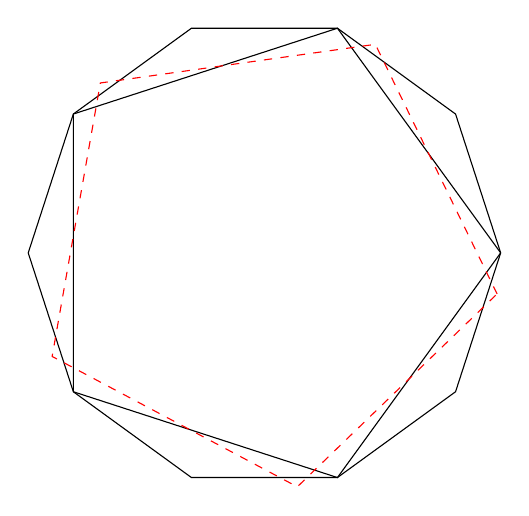
\begin{tikzpicture}[scale = 1.5]
\draw(0:2\R) -- (36:2\R) -- (72:2\R) -- (36*3:2\R) -- (36*4:2\R) -- (36*5:2\R) -- (36*6:2\R) -- (36*7:2\R) -- (36*8:2\R) -- (36*9:2\R) -- (0:2\R);
\draw(0:2\R) -- (72:2\R) -- (36*4:2\R) -- (36*6:2\R) -- (36*8:2\R) --(0:2\R);
\draw[dashed, red] (-10:2\R) -- (72-10:2\R) -- (36*4 - 10:2\R) -- (36*6 -10 :2\R) -- (36*8 - 10:2\R) --(-10:2\R);
\end{tikzpicture}
\end{center}

Notice that each copy of the lamination $L_i$ crosses a copy of the pending arc twice. One of these crossings contributes $+1$ to the shear coordinate and the other crossing contributes $0$, for a net shear coordinate of $+1$. The picture for $b_{\gamma}(T,L_i) = -1$ is analogous.

This extended shear coordinate definition then allows us to apply the usual definition of an elementary lamination to both standard and pending arcs.

Recall that if $\tau_i$ is a standard arc, the corresponding elementary lamination $L_i$ can be found by shifting its endpoints clockwise. Similarly, if $\tau_i$ is a pending arc, then $L_i$ can be found by shifting the singular endpoint clockwise. Examples of both are shown below.

\begin{center}
 \includegraphics[scale=1.5]{Diagrams/elementary_lamination_ordinary.pdf}\qquad
 \includegraphics[scale=2]{Diagrams/elementary_lamination_pending.pdf}
\end{center}

Other types of crossings contribute 0 to the shear coordinate of the pending arc. If we look at these crossings in the cover, they resemble crossings in standard triangulations that contribute~0 to the shear coordinates.

\begin{center}
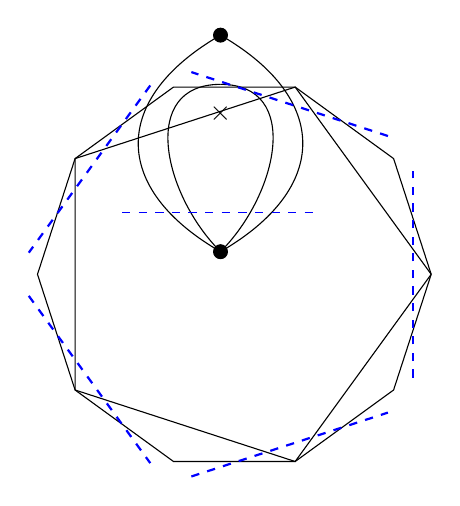
\begin{tikzpicture}[scale = 1.25]

% sets up command for arrows in the middle of arcs
\tikzset{->-/.style={decoration={
 markings,
 mark=at position #1 with {\arrow{>}}},postaction={decorate}}}

%draw exterior boundaries
\draw[out=30,in=-30,looseness=1.5, xshift = -4\R, yshift = -2\R] (0,0.3) to (0,2.5);
\draw[out=150,in=-150,looseness=1.5, xshift = -4\R, yshift = -2\R] (0,0.3) to (0,2.5);

%add pending arc
\draw[in=0,out=45,looseness =1.25, xshift = -4\R, yshift = -2\R] (0,0.3) to (0,2);
\draw[in=180,out=135,looseness=1.25, xshift = -4\R, yshift = -2\R] (0,0.3) to (0,2);

\draw[dashed, blue, xshift = -4\R, yshift = -2\R] (-1, 0.7) -- (1, 0.7);

%draw vertices and orbifold point
\draw[fill=black, xshift = -4\R, yshift = -2\R] (0,0.3) circle [radius=2pt];
\draw[fill=black, xshift = -4\R, yshift = -2\R] (0,2.5) circle [radius=2pt];
\draw[thick, xshift = -4\R, yshift = -2\R] (0,1.7) node {$\mathbf{\times}$};

\draw(0:2\R) -- (36:2\R) -- (72:2\R) -- (36*3:2\R) -- (36*4:2\R) -- (36*5:2\R) -- (36*6:2\R) -- (36*7:2\R) -- (36*8:2\R) -- (36*9:2\R) -- (0:2\R);
\draw(0:2\R) -- (72:2\R) -- (36*4:2\R) -- (36*6:2\R) -- (36*8:2\R) --(0:2\R);
\draw[dashed, blue, thick] (-30: 2.1\R) -- (30: 2.1\R);
\draw[dashed, blue, thick] (-30 + 72: 2.1\R) -- (30+72: 2.1\R);
\draw[dashed, blue, thick] (-30+ 144: 2.1\R) -- (30+144: 2.1\R);
\draw[dashed, blue, thick] (-30-72: 2.1\R) -- (30-72: 2.1\R);
\draw[dashed, blue, thick] (-30-144: 2.1\R) -- (30-144: 2.1\R);
\end{tikzpicture}
\end{center}

However, these new elementary laminations associated to pending arcs will contribute 2 to a standard arc when they cross in a meaningful way. This contribution of 2 is also seen in generalized mutation rules.

\begin{center}
\begin{figure}[h!]
\begin{center}
\begin{tabular}{cc}
 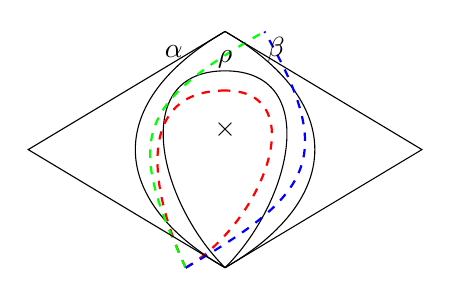
\begin{tikzpicture}[scale = 2.5]
 % sets up command for arrows in the middle of arcs
 \tikzset{->-/.style={decoration={markings, mark=at position #1 with {\arrow{>}}},postaction={decorate}}}

 %draw arcs in triangulation
 \draw[out=30,in=-30,looseness=1.5] (0,0.3) to (0,1.5);
 \draw[out=150,in=-150,looseness=1.5] (0,0.3) to (0,1.5);

 %add pending arc
 \draw[in=0,out=45,looseness =1.25] (0,0.3) to (0,1.3);
 \draw[in=180,out=135,looseness=1.25] (0,0.3) to (0,1.3);

 \draw[in=0,out=30,looseness =1.25, dashed, red, thick] (-0.2,0.3) to (0,1.2);
 \draw[in=180,out=115,looseness=1.25, dashed, red, thick] (-0.2,0.3) to (0,1.2);
 \draw[out = 115, in = 210, dashed, green, looseness = 1.5, thick] (-0.2,0.3) to (0.2, 1.5);
 \draw[out = 30, in = 300, looseness = 1.5, dashed, blue, thick] (-0.2,0.3) to (0.2, 1.5);

 %draw vertices and orbifold point
 %\draw[fill=black] (0,0.3) circle [radius=1pt];
 %\draw[fill=black] (0,1.5) circle [radius=1pt];
 \draw[thick] (0,1) node {$\mathbf{\times}$};

 %adding edge labels
 \node[] at (-0.26,1.4) {$\alpha$};
 \node[] at (0.26,1.41) {$\beta$};
 \node[] at (0,1.36) {$\rho$};

 %Add boundary
 \draw(0,0.3) -- (-1,.9) -- (0,1.5) -- (1,.9) -- (0,0.3);
 \end{tikzpicture} &
 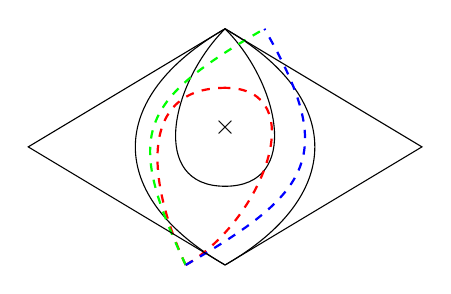
\begin{tikzpicture}[scale=2.5]
 \draw[out=30,in=-30,looseness=1.5, xshift = 3\R] (0,0.3) to (0,1.5);
 \draw[out=150,in=-150,looseness=1.5, xshift = 3\R] (0,0.3) to (0,1.5);

 %add pending arc
 \draw[in=0,out=-45,looseness =1.25, xshift = 3\R] (0,1.5) to (0, 0.7);
 \draw[in=180,out=-135,looseness=1.25, xshift = 3\R] (0,1.5) to (0,0.7);

 \draw[in=0,out=30,looseness =1.25, dashed, red, thick, xshift = 3\R] (-0.2,0.3) to (0,1.2);
 \draw[in=180,out=115,looseness=1.25, dashed, red, thick, xshift = 3\R] (-0.2,0.3) to (0,1.2);
 \draw[out = 115, in = 210, dashed, green, looseness = 1.5, thick, xshift = 3\R] (-0.2,0.3) to (0.2, 1.5);
 \draw[out = 30, in = 300, looseness = 1.5, dashed, blue, thick, xshift = 3\R] (-0.2,0.3) to (0.2, 1.5);

 %draw vertices and orbifold point
 %\draw[fill=black] (0,0.3) circle [radius=1pt];
 %\draw[fill=black] (0,1.5) circle [radius=1pt];
 \draw[thick, xshift = 3\R] (0,1) node {$\mathbf{\times}$};

 %Add boundary
 \draw[xshift = 3\R] (0,0.3) -- (-1,.9) -- (0,1.5) -- (1,.9) -- (0,0.3);
 \end{tikzpicture} \\
 $\begin{bmatrix} 0 & 1 & -1 \\ -1 & 0 & 1 \\ 1 & - 1 & 0 \\ 1 & 0 & 0 \\ 0 & 1 & 0 \\ 0 & 0 & 1 \\ \end{bmatrix}$ & $\begin{bmatrix} 0 & -1 & 1 \\ 1 & 0 & -1 \\ -1 & 1 & 0 \\ 1 & 0 & 0 \\ 0 & 1 & 0 \\ 2 & 0 & -1 \\ \end{bmatrix}$ \\
\end{tabular}
\end{center}
\caption{An example of how flipping a pending arc impacts the shear coordinates of a lamination. The lefthand side of the diagram is an example of an elementary lamination from a triangulated orbifold. This diagram is best viewed in color.}\label{fig:LamFlipPending}
\end{figure}
\end{center}

On the left of Fig.~\ref{fig:LamFlipPending}, we have the elementary lamination associated to this triangulation. When we flip the pending arc, then the lamination associated to the pending arc intersects $\alpha$ nontrivially twice. This matches the result of mutating (with generalized mutation) the extended $B$-matrix associated to the lefthand picture at the index representing the pending arc. The third column and row correspond to the pending arc.

\begin{Remark}
The mutation of the extended portion of the B-matrix resembles the result of mutating at an orbifold point of weight 2 in the sense of \cite{Felikson-Shapiro-Tumarkin}. While the dynamics of our $x$-variables mimic those of orbifold points of weight $\frac12$, the $y$-variables more closely resemble those from orbifold points of weight $2$. This seems to follow from the duality between $c$-vectors and $g$-vectors \cite{NZ}.
\end{Remark}

\section{Constructing snake graphs from orbifolds} \label{Sec:Construction}

In this section, we show how to construct a snake graph (respectively, a band graph) from an arc (closed curve) on a trianguated unpunctured orbifold. Later, we will verify that the weighted sum of perfect matchings gives the correct cluster variable in the case when $\gamma$ is an arc, Theorem~\ref{Thm:GenSnake}, and that for arbitrary $\gamma$, these satisfy skein relations, Proposition~\ref{Prop:OrbSkein}.

\subsection{Tiles}

If $\gamma = \tau_i$ for $1 \leq i \leq n$ (recall the final $c - n$ arcs are boundary arcs), then $G_\gamma$ is a single edge labeled with $\tau_i$. Otherwise, $\gamma$ must cross at least one arc in $T$.

 Let $\tau_{i_1},\ldots, \tau_{i_d}$ be the set of internal arcs of $T$ that $\gamma$ crosses, given a fixed orientation of $\gamma$. For each standard arc $\tau_{i_j}$ that $\gamma$ crosses, we construct a square tile $G_{j}$ by taking the two triangles that $\tau_{i_j}$ borders and gluing them along $\tau_{i_j}$ such that either both either the same orientation relative to $\mathcal{O}$. We say that the square tile produced has relative orientation $+1$ if the orientation of its triangles matches that of $\mathcal{O}$ and $-1$ otherwise. We denote this as $\operatorname{rel}(G_j) = \pm 1.$

\begin{center}
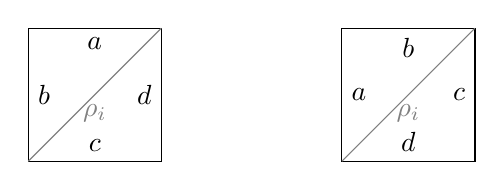
\begin{tikzpicture}[scale = .14cm]
\draw (45:0.3cm) to node[auto]{$a$}(135:0.3cm) to node[auto]{$b$}(180+45:0.3cm) to node[auto]{$c$}(270+45:0.3cm) to node[auto]{$d$} (45:0.3cm);
\draw[gray](45:0.3cm) to node[below]{$\rho_i$} (225:0.3cm);
\draw[xshift = 1 cm] (45:0.3cm) to node[auto]{$b$}(135:0.3cm) to node[auto]{$a$}(180+45:0.3cm) to node[auto]{$d$}(270+45:0.3cm) to node[auto]{$c$} (45:0.3cm);
\draw[xshift = 1 cm, gray](45:0.3cm) to node[below]{$\rho_i$} (225:0.3cm);
\end{tikzpicture}
\end{center}

Next, we consider the case when $\tau_{i_j}$ is a pending arc incident to an orbifold point of order $p$. If $\gamma$ is a generalized arc who shares an endpoint with $\tau_{i_j}$, then it could be that $\gamma$ only crosses~$\tau_{i_j}$ once. In this case, $j = 1$ or $j = k$, and we use a square tile as before. However, the labels of some edges will be given by normalized Chebyshev polynomials, $U_\ell(x)$, evaluated at~$\lambda_p$. Recall $\lambda_p = 2\cos(\pi/p)$.

\begin{Definition} \label{def:Chebyshev}
We let $U_\ell(x)$ denote the $\ell$-th normalized Chebyshev polynomial of the second kind, for $\ell \geq -1$. These are given by initial polynomials $U_{-1}(x) = 0$, $U_0(x) = 1$, and the recurrence, \[
U_\ell(x) = xU_{\ell-1}(x) - U_{\ell-2}(x).
\]
\end{Definition}

For instance, $U_1(x) = x$, $U_2(x) = x^2 - 1$, $U_3(x) = x^3 - 2x$. These polynomials are normalized as they can be recovered by evaluating the standard Chebyshev polynomials of the second kind at~$x/2$.

The following lemma verifies that, up to sign, these labels are independent of increasing or decreasing the winding around an orbifold point by an integer multiple of its order.

\begin{Lemma}\label{lem:ChebyPeriodic}
Evaluations of Chebyshev polynomials at $\lambda_p$ are periodic, in the sense that $U_{k+p}(\lambda_p)\!\allowbreak = -U_{k}(\lambda_p)$. In particular, $U_{p-1}(\lambda_p) = -U_{-1}(\lambda_p) = 0$.
\end{Lemma}

Lemma \ref{lem:ChebyPeriodic} can be readily proven using basic properties of Chebyshev polynomials. We see in Lemmas \ref{lem:Mpathdontcare} and \ref{lem:ChebyshevMatrices} that our statistics are still well-defined up to sign.

The edge labels of these tiles contain $U_\ell(\lambda_p)$ and $U_{\ell - 1}(\lambda_p)$ where $\ell$ is the number of self-intersections of $\gamma$ around the orbifold point. For concision, $U_\ell$ is used as shorthand for $U_\ell(\lambda_p)$ throughout the paper. Moreover, $\alpha$ and $\beta$ may be standard or pending arcs. If one of these arcs is pending, then this is in fact a monogon enclosing two orbifold points.

\begin{center}
\begin{tabular}{|c|c|}
\hline
 \includegraphics[scale=1.5]{Diagrams/SmallPic3.pdf}& \includegraphics[scale=1.5]{Diagrams/SmallPic4.pdf} \\ \hline \includegraphics[scale=1.5]{Diagrams/Small3.pdf} & \includegraphics[scale=1.5]{Diagrams/Small4.pdf} \\ \hline
\end{tabular}
\end{center}

Above, each tile on the left has positive orientation and the tile on the right has negative orien\-tation. We can see this, for example, by comparing the relative orientation of edges labeled~$x_2$ and~$x_a$ with~$\tau_2$ and $\tau_a$.

\begin{Remark}Musiker and Williams discuss a similar example in~\cite{MW} with a puncture rather than an orbifold point. We compare these cases in Section~\ref{sec:RelateToPuncture}.
\end{Remark}

In most cases, if $\gamma$ crosses a pending arc $\tau_{i_j}$, it crosses it twice consecutively, so that $\tau_{i_j} = \tau_{i_{j+1}}$ or $\tau_{i_j} = \tau_{i_{j-1}}$. In this case, we introduce a hexagonal tile which accounts for both intersections. These hexagonal tiles also will have edges labeled by Chebyshev polynomials evaluated at $\lambda_p$, and we again let $\ell$ be the number of self-intersections of $\gamma$ as it winds around the orbifold point. Because these hexagonal tiles can be thought of as ``containing" two square tiles, we assign them a tuple of signs. A hexagonal tile has relative orientation $(+,-)$ if the south-west triangle matches the orientation of the surface and the north-east triangle does not, as on the left hand side of the below diagram, and $(-,+)$ otherwise, as on the right hand side.

\begin{center}
 \includegraphics[scale=1.5]{Diagrams/hexagonalTile.pdf}
\end{center}

In Section \ref{subsec:LiftGenArc}, we give a geometric intuition for why the edge labels $U_\ell\rho$, $U_{\ell+1}\rho$, and $U_{\ell-1}\rho$ appear in this particular arrangement on the hexagonal tiles. This geometric intuition is based on crossing diagonals in the $p$-fold cover. We formally justify these hexagonal tiles in Section~\ref{sec:universalSnakeGraph}, however, using matrix products associated to arcs, perfect matchings of abstract graphs, and Lemma~\ref{lem:ChebyshevMatrices}.

We give puzzle pieces to construct a generalized snake graph from such an arc. Again, $\alpha$~and~$\beta$ could be standard or pending arcs.

\begin{center}
{\renewcommand{\arraystretch}{2}
\begin{tabular}{|@{\,}c@{\,}|@{\,}c@{\,}|@{\,}c@{\,}|@{\,}c@{\,}|}
\hline
 \includegraphics[scale = 2.1]{Diagrams/bigon_case2.pdf} &
 \includegraphics[scale=2.1]{Diagrams/bigon_case2_0winding.pdf} & \includegraphics[scale = 2.1]{Diagrams/bigon_case1.pdf} & \includegraphics[scale=2.1]{Diagrams/bigon_case1_0winding.pdf} \\ \hline \includegraphics[scale = 1.2]{Diagrams/bigon_case2-sg.pdf} & \includegraphics[scale=1.2]{Diagrams/bigon_case2_0winding-sg.pdf} & \includegraphics[scale = 1.2]{Diagrams/bigon_case1-sg.pdf} & \includegraphics[scale=1.2]{Diagrams/bigon_case1_0winding-sg.pdf}
 \\ \hline
\end{tabular}}

\end{center}

Note that if $\ell = 0$ (i.e., the arc does not intersect itself) then the edge labeled $U_{\ell-1}(\lambda_p)$ has weight 0. Thus, we can delete it and recover a standard snake graph with square tiles. We show side by side the general hexagonal tiles and the $k=0$ cases. By Lemma \ref{lem:ChebyPeriodic}, this is also true if $k = p-2$. Moreover, if $\ell = p-1$, then two edges have weight zero and one has negative weight. Using the symmetry of an orbifold point, this is equivalent to not crossing the pending arc at all. Thus, we will assume that $\gamma$ winds less than $p-1$ times around an orbifold point of order~$p$ to avoid including absolute values in our labels.

\subsection[Gluing $G_{T,\gamma}$ puzzle pieces]{Gluing $\boldsymbol{G_{T,\gamma}}$ puzzle pieces}

To construct generalized snake graphs, we will glue together tiles corresponding to arcs crossed consecutively by $\gamma$. If $\gamma$ crosses $\tau_i$ and $\tau_{i+1}$ consecutively, and $\tau_i$ and $\tau_{i+1}$ are distinct arcs, then these arcs form a triangle. Call the third arc in this triangle $\tau_{[i]}$. Then, we glue tiles~$G_i$ and~$G_{i+1}$ along the edge $\tau_{[i]}$. using the appropriate planar embeddings so $\operatorname{rel}(T,G_i) \neq \operatorname{rel}(T,G_{i+1})$. Note that this rule does not differentiate between standard and pending arcs. If~$G_i$ and~$G_{i+1}$ are either both square or both hexagonal, then the statement of the rule is clear. If~$G_i$ is square and~$G_{i+1}$ is hexagonal, then $\operatorname{rel}(T,G_{i+1})$ should be understood to mean the orientation of the south-west triangle of $G_{i+1}$. Likewise, if $G_i$ is hexagonal and $G_{i+1}$ square, then $\operatorname{rel}(T,G_{i})$ should be understood to mean the orientation of the north-east triangle of~$G_i$.

Because the choice of relative orientation for the first tile,~$G_1$, is not fixed, there are two valid planar embeddings of $G_{T,\gamma}$ for any $\gamma$. Our cluster expansion formula produces the same result for either choice of planar embedding, so the choice is unimportant. We also make a choice to glue the tiles so that our snake graphs travel from south-west to north-east; this also will not affect any statistics related to the snake graph.

Finally, we can construct generalized band graphs using the same ideas. Band graphs calculate the length of closed curves on a surface. Choose a point~$p$ on $\gamma$ such that~$p$ does not lie on any arc in $T$ or at an intersection of $\gamma$ with itself. For simplicity, we require $p$ to not be in the interior of a pending arc. Then, construct the snake graph for $\gamma$, picking an orientation and starting and ending at~$p$. Because the first and last tile correspond to arcs bordering the same triangle, they will always have a common edge. We glue the first and tile along this edge, producing a graph which resembles an annulus or a Mobius strip.

Band graphs have the same associated statistics as snake graphs and a version of a perfect matching on a band graph, called a \emph{good matching}, is defined similarly. Musiker and Williams note that a good matching of a band graph can always be obtained from a perfect matching of the original, unglued snake graph used to construct the band graph. To do so, one takes a perfect matching that uses at least one of the glued edges and deletes that glued edge. For further discussion and details, see \cite[Section~3]{MW}.

\subsection{Cluster expansion formulas}

We use Musiker, Schiffler, and Williams' definitions for minimal and maximal matchings, the crossing monomial $\operatorname{cross}(T,\gamma)$, and the weight $x(P)$ and height monomial~$y(P)$ associated to a~perfect matching~$P$, as stated in Section \ref{section:snakeGraphs}. Using this language, we can establish the following theorem for Laurent expansions of arcs (both standard and pending), a more general version of Theorem~4.9 from~\cite{MSW}.

\begin{Theorem}\label{Thm:GenSnake+}
Let $\mathcal{O} = (S,M,Q)$ be an unpunctured orbifold with triangulation $T$ and $\mathcal{A}$ be the corresponding generalized cluster algebra with principal coefficients with respect to $\Sigma_T = (\mathbf{x}_T,\mathbf{y}_T,B_T)$. For an ordinary arc $\gamma$ with generalized snake graph $G_{T,\gamma}$, the Laurent expansion of $x_\gamma$ with respect to $\Sigma_T$ is
\[ [x_\gamma]^{\mathcal{A}}_{\Sigma_T} = \frac{1}{\operatorname{cross}(T,\gamma)} \sum_P x(P)y(P), \]
where the summation is indexed by perfect matchings of $G_{T,\gamma}$.
\end{Theorem}
